\documentclass{article}

\usepackage[utf8]{inputenc}
\usepackage[T1]{fontenc}
\usepackage[french]{babel}



\usepackage{caption}
%\usepackage{pgfplots}
\usepackage{listings}
\usepackage{graphicx}
\usepackage{footnote}
\usepackage{amsmath}
\usepackage{amsthm}
\usepackage{graphicx}
\usepackage{url}
\usepackage{bbm}
\usepackage{amssymb}
\usepackage{mathrsfs}
\usepackage{multirow}
\usepackage{amsfonts}
\usepackage[boxed,linesnumbered,noend]{algorithm2e}
\usepackage{qcircuit}
\usepackage{enumitem}
\usepackage{eurosym}
\usepackage{ulem}

\newtheorem{thm}{Theorem}
\newtheorem{prop}{Propriety}
\newtheorem{lemma}{Lemma}
\newtheorem{defi}{Definition}
\newtheorem{coro}{Corollary}

\newcommand{\deriv}{\mathrm{d}}
\newcommand{\Deriv}{\mathrm{D}}
\newcommand{\grad}{\;\mathrm{grad}\;}
\newcommand{\transpose}{\hspace{.1em}{}^t\hspace{-.1em}}

\setlength{\oddsidemargin}{0pt}
% Marge gauche sur pages impaires
\setlength{\evensidemargin}{0pt}
% Marge gauche sur pages paires
\setlength{\textwidth}{470pt}
% Largeur de la zone de texte 
\setlength{\topmargin}{0pt}
% Pas de marge en haut
\setlength{\headheight}{13pt}
% Haut de page
\setlength{\headsep}{10pt}
% Entre le haut de page et le texte
\setlength{\footskip}{40pt}
% Bas de page + séparation
\setlength{\textheight}{630pt}
% Hauteur de la zone de texte

\title{Introduction à la Mécanique des Milieux Continus}
\author{L. Chamoin\\
ENS Cachan\\
\url{chamoin@ens-paris-saclay.fr}}
\date{}

\newcommand{\note}{\medskip\noindent\underline}

\begin{document}
\maketitle
\tableofcontents
\newpage

\paragraph{Objectifs}
\begin{itemize}
\item Comprendre les enjeux d'étudier les milieu déformables
\item Introduire les concepts de base de la MMC
\item Développer les modèles mathématiques qui en découlent
\item Méthode de résolution numérique et application au HPC
\item Limites de ces modélisations
\end{itemize}
\bigskip

Notation :
\begin{itemize}
\item Deux examens + quelques TD notés
\end{itemize}

Notre professeur fait parti du LMT, un laboratoire du CNRS étudiant des application sur les milieux solides.

\section{Introduction}
Qu'est-ce qu'un milieu continu ? $\to$ milieu physique dans lequel les grandeurs physiques varient de manière continue ("pas de trous"). La notion de milieu continu dépend de l'échelle : par exemple la structure ($\sim 100m-10m$) d'un avion peut être modélisée en utilisant la MMC, mais pas ses cristaux/molécules ($\sim 1 \mu m-1nm$).
\bigskip

La MMC est l'étude des mouvements, déformations et efforts dans les milieux continus avec de nombreuses application (météorologie, aéronautique, conception de bâtiments, ...). Dans ce cours, on s'intéressera principalement à l'aéronautique. Par exemple, pour un avion, il faudra décrire les phénomènes physiques au sein de la matière, les modéliser mathématiquement et les résoudre.

Différentes approches sont possible : de très physique (matériaux) à très mathématique (équations) ou très informatique (logiciels de calcul). Une méthode numérique très utilisée en MMC pour les milieux solides est la \emph{Méthode des éléments finis} ; et la \emph{méthode des cylindres finis} pour les fluides.

L'outil informatique est intéressant pour la résolution de problèmes, qui est la partie la plus dure de la MMC, car à la fois les matériaux utilisés sont complexes, mais la géométrie également ($\to$ non résolvable à la main $\to$ besoin de gros clusters).

La principale différence entre fluide et solide est que les solides se déforment relativement peu.

Au niveau industriels, des logiciels ont été conçu, notamment :
\begin{itemize}
\item ASTER (développé par EDF)
\item CATIA (Dassault)
\item CAST3M (gratuit et en français, développé par le CEA)
\item NASTRAN et ABAQUS : développés par des informaticiens, vendus pour l'industrie
\end{itemize}
Chaque logiciel est plus performant sur une tâche précise.

\subsection{La simulation numérique}
Face à un problème, il faut dans un premier temps réaliser un modèle mathématique théorique (géométrie, comportement, matériaux, ...) puis une maquette numérique (un maillage par exemple) sur lequel sera utilisée la résolution numérique.

Mathématiquement, le problème est régie par des équations aux dérivées partielles, sur lequel ont utilisera la plupart du temps la méthode des éléments finis (informatique).
\bigskip

\paragraph{Historique des simulations numériques}
\begin{itemize}
\item[1850 :] Méthodes analytiques de résolution, assez rudimentaire, résolution manuelle
\item[1940 :] Théorie de la \emph{Méthode des éléments finis}, sans outils informatique cependant (premières applications sur les avions de chasse $\to$ dirigé par l'armée.
\item[1960 :] Utilisation limitée de la simulation, apparition des premiers codes de calcul (NASTRAN)
\item[1980 :] Développement avec l'essor de l'informatique
\item[2000 :] Standardisation
\end{itemize}
\bigskip

En terme de complexité du problème, on parle en nombre d'inconnues. Pour un ordinateur portables, on peut calculer dans un temps raisonnable des problèmes à environ $10^4$ degrés de libertés (ddl). Pour la recherche, les grosses machines peuvent calculer entre $10^6$ et $10^8$ ddl.
\bigskip


La simulation numérique est donc un domaine couvrant à la fois physique (et SI) pour la créations de modèles, mathématiques pour la formulation du problème et les méthode numériques ; et informatique pour la mise en données et les algorithmes de résolution.


\subsection{Applications}
La simulation numérique a de nombreuses applications, pour la physique, biophysique, productique (comment imprimer en 3D de manière optimale ?), etc. Au LMT (laboratoire de mécanique et de technologie) à Cachan, financée à 70\% par airbus.

L'apport de la simulation numérique à l'industrie permet de réduire les essais nécessaire ($\to$ on les simule à la place). Actuellement la simulation numérique est limitée à l'échelle de plusieurs pièces rassemblée ensemble, car on ne peut encore simuler un assemblage complexe, ni contrôler la marge d'erreur. On tends aujourd'hui à développer la simulation, car elle permet d'économiser de l'argent (pas besoin de pièces) et du temps.


\paragraph{Utilité des modèles} \emph{Essentially, all models are wrong, but some are useful}

Une modélisation ne sera jamais conforme à la réalité, mais on peut borner l'erreur. On peut par exemple contrôler l'erreur que l'on fait en modifiant le maillage.


\section{Cinématique des milieux continus}
Il s'agit de l'étude des mouvement des points de la matière du milieu.

\subsection{Repérage en mécanique du point}
\begin{itemize}[label=\textbullet]
\item Temps $t$
\item Référentiel (ou observateur)
\item Vecteur position $t \mapsto \overrightarrow{OM}(t)$
\item Vitesse $\vec{v}$ : $t \mapsto \vec{v}(M,t) = \dfrac{\deriv \overrightarrow{OM}}{\deriv t}$
\item Accélération $\vec{a}$ : $t \mapsto \vec{a}(M,t) = \dfrac{\deriv^2 \overrightarrow{OM}}{\deriv t}$
\end{itemize}

\subsection{Notion de milieu continu}
Le milieu évolue avec le temps, en chaque point du milieu on peut utiliser les méthodes de repérage ponctuelles. Le milieu continue est un ensemble infini de points !

Deux visions existent : la vision \emph{Lagrangienne} et \emph{Eulérienne}.

\subsubsection{Vision lagrangienne}
La vision Lagrangienne est la plus utilisée par les solides, on étudie le mouvement du solide par rapport à sa position initiale déterminée appelée \emph{configuration de référence}. Elle consiste en la donnée pour tout temps et tout point $M_0$ du solide $\Omega$ de configuration initiale $\Omega_0$ la trajectoire $\overrightarrow{OM}_0(t)$.

Tout est donnée par rapport à la position initiale. On suit chaque point, donc $\vec{a}=\dfrac{\deriv \vec{v}}{\deriv t}$


\subsubsection{Vision Eulérienne}
Elle est la plus utile en mécanique des fluides. En effet pour un fluide, on ne sait pas exactement d'où la particule est partie. On se donne alors pour tout point $M(x,y,z)$ du milieu la vitesse $v(t,x(t),y(t),z(t))$. Dans ce cas
\begin{align*}
\vec{a}_M (t) & = \dfrac{\Deriv \vec{v}}{\Deriv t}\\
& = \dfrac{\partial \vec{v}_M(t)}{\partial t} + \vec{v} \grad \vec{v}
\end{align*}


\subsection{Déformation}
Cela signifie que la distance entre les points change. En vision lagrangienne, soit $M_0$ et $N_0$ appartenant à $\Omega_0$. Le vecteur $\overrightarrow{M_0N_0}$ évolue pour donner $\overrightarrow{MN}(t)$ donnant la déformation de la matière en fonction du temps.

On pose :
\begin{align*}
\overrightarrow{MN} & = \overrightarrow{ON} - \overrightarrow{OM}\\
& = \underbrace{\overrightarrow{ON}(t,\overrightarrow{ON}_0}_{\vec{\Phi}(t,\overrightarrow{ON}_0)} - \underbrace{\overrightarrow{OM}(t,\overrightarrow{OM}_0}_{\vec{\Phi}(t,\overrightarrow{ON}_0}\\
& = \vec{\Phi}(t, \overrightarrow{OM}_0 + \overrightarrow{M_0N_0}) - \vec{\Phi}(t, \overrightarrow{OM}_0)\\
& = \underbrace{\dfrac{\partial \vec{\Phi}}{\partial M_0}}_{= \mathbb{F}} (\overrightarrow{M_0N_0}) + ... \qquad \text{(développement limité)}
\end{align*}

On note $\mathbb{F}$ la \emph{matrice gradient de la transformation}, qui dépend de $t$ et de $M_0$. 
Par l'intermédiaire de $\mathbb{F}$, on peut déduire l'évolution d'un petit volume de matière $V_0$ :  $V = V_0 \cdot \det (\mathbb{F})$

Pour qualifier le \emph{cisaillement} (c'est à dire le fait que l'objet ne fait pas que tourner sur lui-même par exemple, mais que les angles évoluent). On utilise alors la \emph{matrice de déformation} $\mathbb{E}$. On parle aussi de \emph{tenseurs}.

\[\mathbb{E} = \dfrac{1}{2} \left ( \mathbb{F} \transpose\mathbb{F} - \mathbb{I} \right ) \in \mathscr{S}_3(\mathbb{R})\]

Les coefficients diagonaux correspondent à l'allongement :
\begin{align*}
\mathbb{E}_{11} & = \vec{x}\mathbb{E}\vec{x}\\
& = \dfrac{1}{2} \; \hdots\\
& = \dfrac{1}{2\ell_0 ^2} \left ( \ell - \ell_0^2 \right )
\end{align*}
Avec $\ell_0$ la longueur originale du vecteur infinitésimal $\overrightarrow{M_0A_0}$ selon $Ox$.
\bigskip

De même, les coefficients hors-diagonale quantifient le \emph{glissement} (ou \emph{rotation}) :
\begin{align*}
\mathbb{E}_{12} & = \vec{y}\transpose \mathbb{E} \vec{x}\\
& = ... \\
& = \dfrac{\Delta \ell}{2 \Delta_0 \ell_0} \cos \alpha
\end{align*}
Avec $\Delta_0$ la longueur originale du vecteur infinitésimal $\overrightarrow{M_0B_0}$ selon $\vec{y}$ et $\alpha$ l'angle entre $\overrightarrow{MA}$ et $\overrightarrow{MB}$. A $t=0$, $\alpha = \dfrac{\pi}{2}$.

\paragraph{Exemple} 

\begin{enumerate}
\item
Un cylindre en translation selon $\vec{x}$.

\begin{align*}
\overrightarrow{OM}_0 \left\lvert \begin{matrix}
x_0\\
y_0\\
z_0\\
\end{matrix} \right. \longmapsto 
\overrightarrow{OM}(t) \left\lvert \begin{matrix}
x(t) = x_0 + b(t)\\
y(t) = y_0\\
z(t) = z_0\\
\end{matrix} \right.
\end{align*}

On trouve $\mathbb{E} = \begin{pmatrix}
1 & 0 & 0 \\
0 & 1 & 0 \\
0 & 0 & 1 \\
\end{pmatrix}$ $\to$ pas de déformation.

\item 
Un cylindre en rotation d'axe $Oz$

\begin{align*}
\overrightarrow{OM}_0 \left\lvert \begin{matrix}
x_0\\
y_0\\
z_0\\
\end{matrix} \right. \longmapsto 
\overrightarrow{OM}(t) \left\lvert \begin{matrix}
x(t) = x_0 \cos\theta - y_0\sin \theta\\
y(t) = x_0\sin\theta + y_0\cos \theta\\
z(t) = z_0\\
\end{matrix} \right.
\end{align*}

On trouve 
\[ \mathbb{F} = \begin{pmatrix}
\cos\theta & -\sin\theta & 0\\
\sin\theta & \cos\theta & 0\\
0 & 0 & 1\\
\end{pmatrix}
\]

et
\[\mathbb{E} = \mathbb{I}_3\]


\item
Soit un carré de matière de côté $\eta$, avec $\vec{v}(M_0)=\alpha \left\lvert \begin{matrix}
y_0\\0\\0
\end{matrix}\right. $ (il s'étale en formant un parallélogramme à volume constant).

Dans ce cas, on trouve : 
\[\mathbb{F} = \begin{pmatrix}
1 & \alpha t & 0\\
0 & 1 & 0\\
0 & 0 & 1
\end{pmatrix}
\]

et

\[\mathbb{E}= \begin{pmatrix}
0 & \alpha t & 0\\
\alpha t & (\alpha t)^2 & 0\\
0 & 0 & 0
\end{pmatrix}
\]
Ce qui est cohérent physiquement : les longueurs sur $Oy$ varient, et tout comme les angles avec ce dernier.

\item Soit un carré de côté $\eta$ avec $\vec{v}(M_0)=\alpha \left\lvert \begin{matrix}
y_0\\-x_0\\0
\end{matrix}\right.$ (il tourne tout en s'agrandissant mais garde sa forme).


On trouve :
\[\mathbb{F} = \begin{pmatrix}
1 & \alpha t & 0\\
-\alpha t & 1 & 0\\
0 & 0 & 1\\
\end{pmatrix}
\]
et
\[
\mathbb{E} = \dfrac{1}{2}\begin{pmatrix}
(\alpha t)^2 & 0 & 0\\
0 & (\alpha t)^2 & 0\\
0 & 0 & 0\\
\end{pmatrix}
\]
Ce qui est également physiquement cohérent : les angles (coefficients hors diagonales) ne varient pas, mais les longueurs sur $Ox$ et $Oy$ augmentent avec $t$.
\end{enumerate}

\subsubsection{Vision Lagrangienne}
Outre $\mathbb{F}(t,M_0)$ et $\mathbb{E}(t, M_0)$, on introduit le \emph{déplacement} $\vec{u}$, défini par $\overrightarrow{OM}=\overrightarrow{OM_0}+\vec{u}$. On a alors $\mathbb{F}= \mathbb{I} + \grad_{| M_0} \vec{v}$

Dans ce cas :
\begin{align*}
\mathbb{E} & = \dfrac{1}{2}[\mathbb{F}\transpose \mathbb{F} - \mathbb{I}]\\
& = \dfrac{1}{2} \left[ \underbrace{(\mathbb{I} + \grad \vec{u})\transpose(\mathbb{I}+\grad \vec{v}) - \mathbb{I})}_{= \mathbb{I}+ \grad \vec{u} + \transpose \grad \vec{u} + \underbrace{\text{\sout{$\transpose \grad \vec{u}\grad \vec{u}$}}}_{\substack{\text{négligé pour les solides}\\\text{avec de petites déformations}}}} \right]\\
& \simeq \underbrace{\dfrac{1}{2} \left[ \grad_{M_0} \vec{v} + \transpose \grad_{M_0} \vec{v} \right]}_{\varepsilon (\vec{u})\text{ déformation linéarisée}}\\
\end{align*}

\paragraph{Note}
$\mathbb{F}$,$\mathbb{E}$ et $\varepsilon$ sont des composants sans unité, de l'ordre de $10^{-6}$ à $10^{-3}$.

\subsubsection{Vision eulérienne}
Pour avoir une idée de la déformation dans le milieu, on introduit
\[\mathbb{D} = \dfrac{1}{2} \left[ \grad_M \vec{v} + \grad_M \vec{v} \right]\]
Avec $\dfrac{\deriv  \overrightarrow{MN}}{\deriv t} = \mathbb{D} \cdot \overrightarrow{MN}$. $\mathbb{D}$ est appelé \emph{tenseur taux de déformation}, son unité est la $s^{-1}$.


\paragraph{Exemple} $\vec{v}(M,t) = \left\lvert \begin{matrix}
v_x = \omega y\\
v_y = \omega x + a\omega^2 t\\
0
\end{matrix}\right.$


Passage à une vision lagrangienne $\to$ retour à la notion de trajectoire
\begin{align*}
v_x & = \omega y = \dfrac{\deriv x}{\deriv t}\\
v_y & = -\omega x + a\omega^2 t = \dfrac{\deriv y}{\deriv	t}\\
v_z & = 0 = \dfrac{\deriv z}{\deriv t} \Rightarrow z(t) = z_0
\end{align*}

On se retrouve avec deux équations différentielles :
\begin{align*}
& \dfrac{\deriv^2 y}{\deriv t ^2} + \omega^2 y = a \omega^2\\
\Rightarrow & \begin{cases}
y(t) = a + K_1\cos \omega t + K_2\sin\omega t\\
x(t) = -\dfrac{1}{\omega}(-K_1 \omega \sin \omega t + K_2 \cos \omega t) + a \omega t)
\end{cases}
\end{align*}

\section{Représentation des efforts dans la matière}
\subsection{Classifications des efforts}
Le vrai mot serait plutôt "action mécanique". On parle :
\begin{itemize}[label=\textbullet]
\item D'efforts extérieurs surfaciques $\to$ densité surfacique $\vec{F}_d$ en $N.M^{-2}$, par exemple la pression (attention, elles ne sont pas toujours orthogonales à la surface !)
\item D'efforts extérieurs volumiques $\to $ densité volumique $\vec{f}_d$ en $N.m^{-3}$.
\item D'efforts intérieurs surfaciques, en $N.m^{-2}$.
\end{itemize}

\subsection{Effort de cohésion : notion de contrainte}
Soit une surface élémentaire $\deriv S$ de normale $\vec{n}$. Il a été montré (Cauchy) que l'effort s'appliquant dessus $\deriv \vec{F}$ (en $N$) se décompose en $\deriv \vec{F} = \deriv S \times \vec{T} (M,\vec{n})$ où $\vec{T}$ est appelé \emph{vecteur contrainte} en $N.m^{-2}$. Il a également été prouvé $\vec{T}(M,\vec{n})=\sigma (M).\vec{n}$ où $\sigma$ est une matrice (tenseur) des contraintes. 

\subsubsection*{Quelques propriétés}
$\sigma$ est symétrique (cela vient du fait que le système est à l'équilibre).

\paragraph{Exemple} Traction pure : on étire de chaque côté une barre. Dans ce cas,
\[\sigma(M) = \begin{pmatrix}
\sigma_0 & 0 & 0\\
0 & 0 & 0\\
0 & 0 & 0\\
\end{pmatrix}_{(\vec{e}_1, \vec{e}_2, \vec{e}_3)}\]
\bigskip
De la même manière que $\mathbb{E}$, les coefficients diagonaux représentent les \emph{tractions} et les coefficients non-diagonaux le \emph{cisaillement}.
$\sigma$ étant symétrique, on peut la diagonaliser :
\[\sigma(M) = \begin{pmatrix}
\sigma_I & 0 & 0\\
0 & \sigma_{II} & 0\\
0 & 0 & \sigma_{III}
\end{pmatrix}_{(e_I, e_{II}, e_{III})}
\]

Les coefficients diagonaux sont appelés \emph{contraintes principales} et la base \emph{base principale}.


\subsection{Pression hydrostatique}
Une bille dans l'eau : $\sigma = -p \mathbb{I}$


\paragraph{Ordre de grandeurs} $|| \sigma || \sim 100$ MPa


\paragraph{Écrasement d'un solide entre deux plaques rigides} On suppose qu'il y a glissement sur la plaque du bas mais frottement dur la plaque supérieure.
\begin{figure}[!h]
\centering
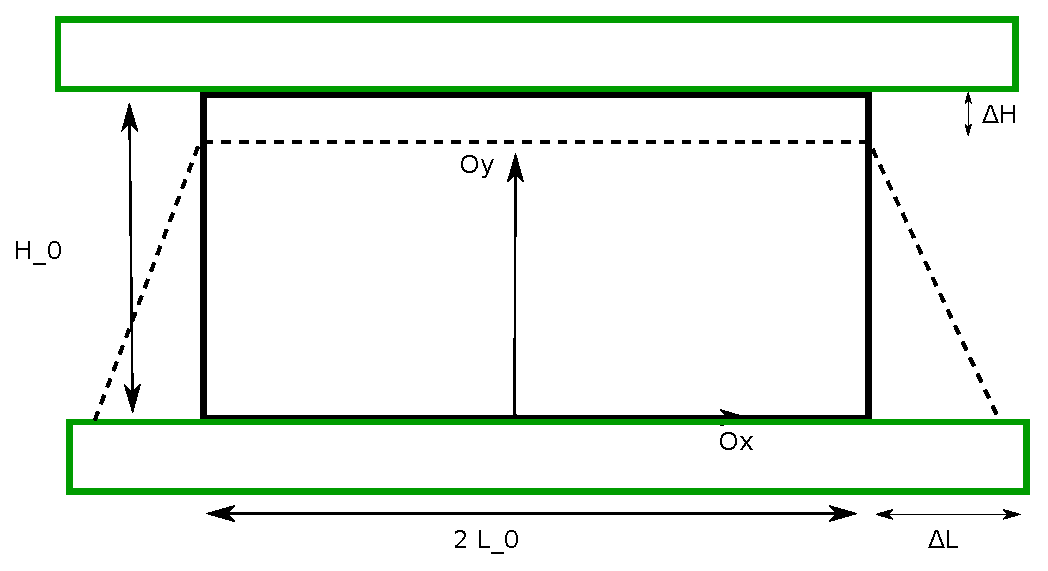
\includegraphics[width=0.6\linewidth]{deux_plaques.eps}
\end{figure}

On trouve :
\[\mathbb{E} = \dfrac{1}{2}\begin{pmatrix}
\left(1 + \dfrac{\Delta L}{L_0}\left(1-\dfrac{\Delta H}{H_0}\right)\right)^2 - 1 &
- \left(1 + \dfrac{\Delta L}{L_0}\left(1-\dfrac{\Delta H}{H_0}\right)\right) x_0 \dfrac{\Delta L}{L_0 H_0} & 0 \\
\times & \left(x_0\dfrac{\Delta L}{L_0}\right)^2 + \left(1 -\dfrac{\Delta H}{H_0}\right)^2 - 1 & 0\\
\times & \times & 0\\
\end{pmatrix}
\]

Et
\[ \varepsilon (\vec{u}) = 
\begin{pmatrix}
\dfrac{\Delta L}{L_0}\left(1-\dfrac{y_0}{H_0}\right) & -\dfrac{x_0}{2}\dfrac{\Delta L}{L_0 H_0} & 0\\
\times & -\dfrac{H}{H_0} & 0\\
\times & \times & 0
\end{pmatrix}
\]

Ce qui correspond à considérer que les mouvements sont petits ($\Delta H \ll H_0$ et $\Delta L \ll H_0$).

\subsection{Notion de contrainte}
Elle est particulièrement adaptée à une version eulérienne, il existe un autre outil (matrice de Piola).
\bigskip

Une surface élémentaire $\deriv S$ subit une force $\overrightarrow{\deriv F} = \deriv S . \vec{T}(M,\vec{n})$ où $\vec{T}=\mathbb{\sigma}(M).\vec{n}$ avec $\mathbb{\sigma}$ la matrice des contraintes.

\paragraph{Exercice}
\begin{enumerate}
\item (2.4 de la fiche) 
Essai de traction dans une éprouvette d'essai de traction cylindrique de rayon $R$.\\
Attention à bien orienter la normale en fonction de quelle matière effectue son effort sur qui (cela change le signe). Le chargement extérieur est $p_0 S_0 \vec{e}_1$, donc $\vec{T}(M,\vec{e}_1)=\rho_0 \vec{e}_1$. La section étudiée est une ellipse d'inclinaison $\theta$ par rapport à  une section verticale. Sa surface est donc $\pi \dfrac{R^2}{\cos \theta}$. Sur cette ellipse, on a alors $\vec{T}(M,\vec{n}=\dfrac{p_0 S_0 \vec{e}_1}{S_1}=p_0\cos \theta \vec{e}_1$.

En fait, puisqu'on a une traction selon $\vec{e}_1$, on pouvait directement dire que
\begin{align*}
\vec{T}(M,\vec{n}) & = \sigma (M).\vec{n}\\
& = \begin{pmatrix}
p_0 & 0 & 0 \\
0 & 0 & 0\\
0 & 0 & 0\\
\end{pmatrix} . \vec{n}
\end{align*}

D'un point de vu physique, on peut différencier l'effort \emph{normal} et l'effort \emph{tangentiel}. Ici, on trouve un effort normal de $p_0\cos^2 \theta$ et un effort tangentiel de $p_0 \dfrac{\sin (2\theta)}{2}$ (avec un peu de trigo...), maximal quand $\theta = \dfrac{\pi}{2}$ ce qui explique pourquoi les matériaux sensibles au cisaillement cassent avec un plan de cassure à $45^\circ$.

\item Essai de bi-traction : on exerce une pression uniforme $\sigma_1$ selon $\vec{e}_1$ et $\sigma_2$ selon $\vec{e}_2$.

\begin{align*}
\sigma & =
\begin{pmatrix}
\sigma_1 & 0 & 0\\
0 & \sigma_2 & 0\\
0 & 0 & 0\\
\end{pmatrix}\\
\vec{T}(M,\vec{n}) = \sigma.\vec{n} & =
\begin{pmatrix}
\sigma_1 & 0 & 0\\
0 & \sigma_2 & 0\\
0 & 0 & 0\\
\end{pmatrix}
\cdot
\begin{pmatrix}
\cos \theta\\
\sin \theta\\
0\\
\end{pmatrix}
=
\begin{pmatrix}
\sigma_1 . \cos \theta\\
\sigma_2 . \cos \theta\\
0\\
\end{pmatrix}
\end{align*}

On trouve
\[\vec{T}(M,\vec{n}) = [\sigma_1 \cos^2 \theta + \sigma_2 \sin^2 \theta] \vec{n} + [(\sigma_2-\sigma_1)\cos \theta \sin \theta]\vec{t}\]
Ceci forme le cercle de Mohr.

\end{enumerate}


\subsection{Équations de conservation}
Elles pilotent l'évolution de l'état de la matière (déformation, contraintes).

\subsubsection{Conservation de la masse}
\paragraph{Vision lagrangienne}
\[n_0 = \int_{\omega_0} \rho_0 \deriv v_0 = \int_{\omega} \deriv v\Rightarrow \rho_0 = \rho. \det \mathbb{F}\]

\paragraph{Vision eulérienne}
\[\dfrac{\deriv}{\deriv t} \int_{\omega(t)} \rho (L,t) \deriv v = 0\]
Dont on extrait :
\[\dfrac{\partial \rho}{\partial t}+\text{div} (\rho \vec{v}) = 0\]
Pouvant se simplifier :
\begin{align*}
\text{Cas stationnaire : }& \text{div} (\rho \vec{v}) = 0\\
\text{Cas incompressible : }& \dfrac{\deriv \rho}{\deriv t} = 0 \to \text{div} \vec{v} = 0\\
\end{align*}

\subsubsection{Conservation de la quantité de mouvement (équilibre de la matière)}

Si $\omega$ est un volume et $\gamma$ sa frontière.

\[\int_{\omega(t)} \vec{f} \deriv v + \int_{\gamma} \vec{T}(M,\vec{n}) \deriv S \]
Que l'ont peut réécrire en
\[ \overrightarrow{\text{div}}\; \sigma + \vec{f} = \rho \cdot \dfrac{\deriv \vec{v}}{\deriv t} (=0 \text{ en statique})\]

Noter qu'il existe aussi une équation de conservation de l'énergie $\to$ pas traité ici.

\paragraph{Exemple :}
Un cube sur un plan subissant uniquement son poids propre.
On suppose 
\[\sigma(M) = 
\begin{pmatrix}
0&0&0\\
0&0&0\\
0&0&a+bz\\
\end{pmatrix}
\]

On trouve alors $\sigma_{33} = \rho . g . (z-H)$.


\subsubsection{Comportement du matériau}
\paragraph{Idée} Trouver un lien entre $\mathbb{E},\varepsilon, \mathbb{D}$ et $\sigma$.

\paragraph{Cas d'un solide (en petite perturbation) :} $\sigma(M) = f_{M}(\varepsilon(M))$
\begin{itemize}[label=$\star$]
\item Aspect homogène/hétérogène : dépendance avec la \textit{position} du point $M$.
\item Aspect isotrope/anisotrope : dépendance du comportement avec l'\textit{orientation}. Si le matériau est isotrope, $\sigma = f(\varepsilon, \text{Tr}(\varepsilon), \text{Tr}(\varepsilon^2), \text{Tr}(\varepsilon^3))$
\end{itemize}

\begin{itemize}
\item Cas d'un matériau élastique : Pas de notion de mémoire, et $\varepsilon_{ii} = \dfrac{\Delta \ell}{\ell_0}$ ($\varepsilon_{ii}$ coefficient de $\varepsilon$ dans la direction de l'élongation).\\
Dans le cas d'un élastique linéaire : $\sigma = K\cdot\varepsilon$, ou $K$ est un \emph{tenseur d'ordre 4} (dit tenseur d'élasticité de Hooke, $K_{ijkl}$, alors que $\sigma$ et $\varepsilon$ sont des matrices carrées d'ordre 3). $K$ a donc $3^4=81$ coefficients, mais par symétrie on se ramène à $21$ coefficients indépendants. Il peut y avoir des symétries :
\begin{itemize}[label=\textbullet]
\item Matériaux orthotrope : 3 plans de symétrie orthogonaux $\to$ 9 coefficients
\item Matériaux isotropes transverse : (matériaux en couches) $\to$ 4 coefficients
\item Matériaux isotropes : 2 coefficients : $E,\nu$ $\to$ $E=$ module d'Young et $\nu=$coefficients de Poisson ; ou (autre représentation) $\lambda,\mu$ coefficients de Lamé

Dans ce cas, on a $\sigma = 2\mu \varepsilon + \lambda \text{Tr}(\epsilon) \mathbb{I}$ avec $2\mu = \dfrac{E}{1+\nu}$ et $\lambda = \dfrac{\nu E}{(1+\nu)(1-2\nu)}$. Noter que si $\nu = 0,5$, alors le matériau est incompressible.

Pour
\[
\sigma = \begin{pmatrix}
\tilde{\sigma} & 0 & 0\\
0 & 0 & 0\\
0 & 0 & 0\\
\end{pmatrix}
\]
Alors 
\[\varepsilon = 
\begin{pmatrix}
\dfrac{\tilde{\sigma}}{E} & 0 & 0\\
0 & -\dfrac{\nu}{E}\tilde{\sigma} & 0\\
0 & 0 & -\dfrac{\nu}{E}\tilde{\sigma}
\end{pmatrix}
\]
\paragraph{Ordre de grandeur :}
\begin{itemize}[label=$\star$]
\item $\varepsilon \sim 1^{-3}-10^{-6}$
\item $\tilde{\sigma}\sim 0-100$ MPa
\item $E \simeq 100$ GPa
\item $\nu \sim 0,2 - 0,3 < 0,5$ (peut etre négative pour certaines micro-structures spécifiques (on tire dessus et tout s'allonge).
\end{itemize}
\end{itemize}
\end{itemize}

\paragraph{Cas d'un fluide :}
\begin{itemize}
\item fluide parfait : $\sigma = -p . \mathbb{I}$, où $p$ est la pression. Il n'y a alors pas de contrainte tangentielle donc pas de viscosité.
\item fluide newtonien : $\sigma = -pI + 2 \mu D + \underbrace{\lambda \text{Tr}[D].\mathbb{I}}_{\text{si incompressible}}$
\end{itemize}

\section{Écriture d'un problème de MMC}
Pour un problème fluide de volume $\omega$ et surface $\gamma$, on utilise :
\begin{align*}
\dfrac{\partial \rho}{\partial t} + \text{div}(\rho \vec{v}) & = 0\\
\overrightarrow{\text{div}}\sigma + \vec{f} & = \rho\dfrac{\deriv \vec{v}}{\deriv t}\\
\sigma & = -p\mathbb{I} + 2 \mu \mathbb{D} \quad ( + \lambda \text{Tr}[\mathbb{D}] \mathbb{I})
\end{align*}
Et les conditions aux limites (valeurs de $\vec{v}$ ou $\sigma \vec{n}$ sur $\gamma$).
\bigskip

Pour les solides dans le modèle des petites perturbations ($\rho_0 = \rho \det \mathbb{F}$) :
\begin{align*}
\overrightarrow{\text{div}} \sigma + \vec{f} & = \Big(\rho \dfrac{\deriv \vec{v}}{\deriv t} \Big)\\
\sigma & = 2\mu\varepsilon (\vec{u}) + \lambda \text{Tr}[\varepsilon(\vec{u})]\mathbb{I}
\end{align*}
Ainsi que les conditions aux limites.

\paragraph{Résolutions}
\begin{itemize}[label=$\star$]
\item On intuite une forme pour $\vec{u}, \vec{v}, \sigma$.
\item On regarde si on peut vérifier toutes les équations. Si non, on revient à l'étape précédente. 
\end{itemize}

\paragraph{Exemple :}
\begin{enumerate}
\item Écoulement dans une conduite cylindrique d'axe $Oz$. On suppose que $\vec{v}=v(r).\vec{e}_z$, et que l'ont est en régime stationnaire.

En reprenant les équations antérieures : 
\begin{align*}
\text{div}(\vec{v}) = 0\\
\overrightarrow{\text{div}}\dfrac{\deriv \vec{v}}{\deriv t}=\rho [\dfrac{\partial \vec{v}}{\partial t} + (\nabla \vec{v})\vec{v}]\\
\sigma = -p \mathbb{I} + 2\mu \mathbb{D}\\
\vec{v}=\vec{0} \text{ en } r=R\\
p(z=0)=p_0\\
p(z=L)=p_L\\
\end{align*}

\item Un matériau élastique cylindrique linéaire isotrope homogène $(E,\nu)$ (ou $(\lambda, \mu)$), possédant une pression interne, et statique.
\begin{align*}
\overrightarrow{\text{div}}\sigma = \vec{0}\\
\sigma = 2\mu \varepsilon(\vec{u}) + \lambda \text{Tr}[\varepsilon(\vec{u})] \mathbb{I}\\
\sigma \vec{n}=\vec{0} \text{ sur les bords } S_0,S_H\\
\sigma \vec{n}=p_i\vec{e}_r \text{ sur } S_{int}\\
\end{align*}



\end{enumerate}



\end{document}
